\chapter{Problem Statement}

%Implementation of an immediate file in MINIX 3 file system, which will help in saving space and improve the %performance for small files. Files smaller than 32 Bytes can be accommodated in the inode itself which is usually %used to store the pointers to disk block. 
\vspace{10mm}

\large Understand the VFS and implement support for Immediate Files in Minix Filesystem. \\

\textbf{What are Immediate Files ?}

Immediate files are basically storage for small files where the data is stored directly in the inode, without the need to traverse pointers to external blocks. Let's first review how file systems work in Minix:

Each regular Minix file is represented by an inode that stores metadata about a file (such as file size or the user id of file owner), as well as the number of disk blocks that store the file's content. To find the disk blocks storing the file content, an inode also stores pointers (in the inode's i\_zone array). These pointers can either point directly to a disk block storing data, or to a block that stores a list of additional pointers to data blocks (indirect blocks). But for really small files, say 1 or 2 byte files, a complete disk block still needs to be allocated. In Minix, these blocks are generally called Zones, but it's the same thing. Because each block or zone has a minimum size of 4KB, this clearly wastes a lot of space.

To make storage more efficient for small files, and to reduce internal fragmentation, we can use immediate files. An immediate file is a file whose data is not stored in a data block, but directly inside the inode itself. An inode in Minix is 64 bytes long, and 40 bytes are used to hold pointers to data blocks. For immediate files, you can clearly use those 40 bytes to store the file contents instead of pointers. 
\begin{center}
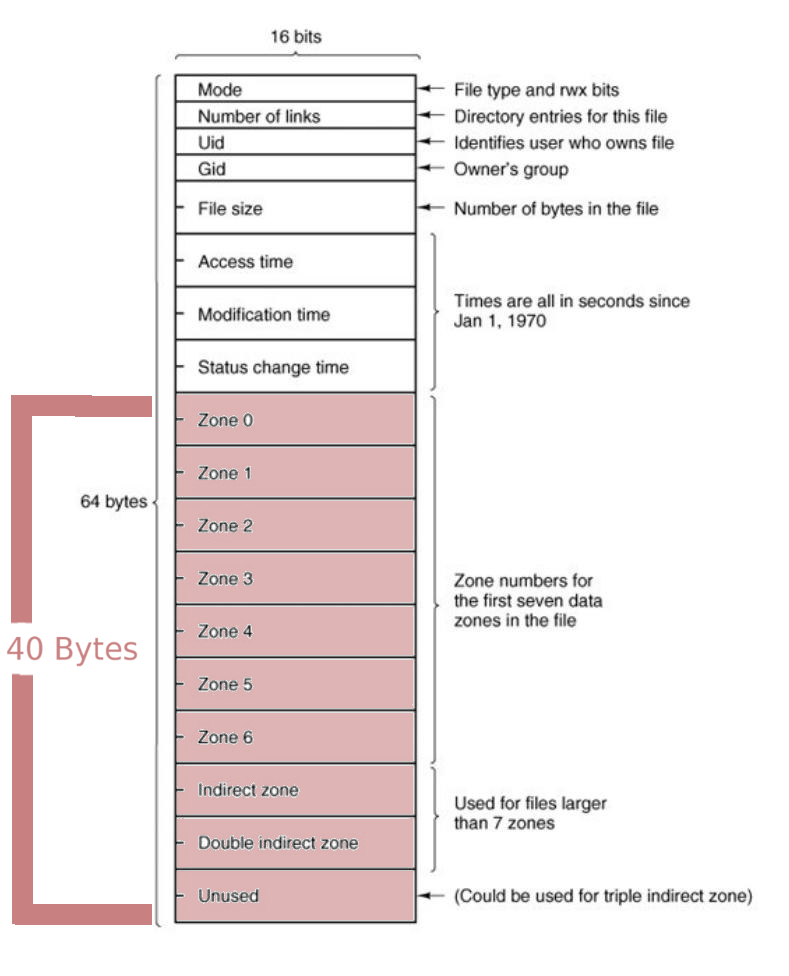
\includegraphics[scale=.5]{pics/inode.jpg} 
\end{center}
In the above picture the colored portions indicate the space used to save disk block pointers in inode structure. Our job is to utilize this space and implement immediate files.

Immediate file was proposed by Andrew S. Tanenbaum and Spaje J. Mullender in 1984\cite{astimme}.


 {\bf Specifications}:\\
\begin{itemize}
\item An Immediate file is created only when we pass an open flag O\_CREATI (you will have to define this open flag constant).
\begin{itemize}
\item by default we use open system calls to create a regular file:
    open("filename", O\_CREAT , 0666);
    
\item  now for creating immediate file we will define a new constant O\_CREATI and open system call with parameter O\_CREATI should create an immediate file:
    open("filename", O\_CREATI, 0666);   
\end{itemize}

\item All other file operations (open, delete, read, write ...) should work on immediate files.
\item When size of immediate file reaches 32 Bytes the filesystem should return an error. 

\end{itemize}


